\documentclass[../notes.tex]{subfiles}

\pagestyle{main}
\renewcommand{\chaptermark}[1]{\markboth{\chaptername\ \thechapter\ (#1)}{}}

\begin{document}




\chapter{A Rigorous Definition of Symmetry}
\section{Symmetry: Symmetry Elements and Operations}
\begin{itemize}
    \item \marginnote{9/28:}Dr. Anna Wuttig (AH-nuh WUH-tig).
    \begin{itemize}
        \item Teaches exclusively on the blackboard.
        \item Will record lectures, however; if there is a technical error, she will upload last year's lecture.
    \end{itemize}
    \item Syllabus.
    \begin{itemize}
        \item PSets graded on completion, not accuracy.
        \item Two exams: One on the first half of the course; one on the second half of the course.
        \begin{itemize}
            \item Cumulativeness: You'll need to understand the first half to do the second half, but there won't be questions specifically targeted to first-half material.
        \end{itemize}
        \item No final.
        \item Participation. Showing up to class and working in groups.
    \end{itemize}
    \item Chris, Dan, Amy, Matt, Jintong, Yibin, Ben, Sara, Ryan, Joe, Owen, Isabella, Pierce are the people.
    \begin{itemize}
        \item People come from a diversity of chemistry subfields (physical, inorganic, organic, materials, biological).
    \end{itemize}
    \item Every day will have a handout that we will write on (in pencil).
    \item Study the learning objectives!
    \item (Local) symmetry of a molecule helps us predict and describe bonding, spectroscopic properties, and reactivity.
    \begin{itemize}
        \item We describe symmetry with group theory.
    \end{itemize}
    \item \textbf{Symmetry operation}: An operation which moves a molecule into a new orientation equivalent to its original one (geometrically indistinguishable).
    \begin{itemize}
        \item Symmetry operations that can be applied to an object always form a \textbf{group}.
    \end{itemize}
    \item \textbf{Symmetry element}: A point, line, or plane about which a symmetry operation is applied.
    \item Symmetry operations.
    \begin{enumerate}
        \item Identity operation ($E$): Do nothing; null operation.
        \item Reflection through a plane ($\sigma$): Subdivided into\dots
        \begin{itemize}
            \item $\sigma_d$: \underline{d}ihedral mirror planes, which contain the principle $C_n$ axis and bisect the angles formed between adjacent $C_2$ axes;
            \item $\sigma_h$: \underline{h}orizontal mirror planes, in which the mirror plane is perpendicular to the principal $C_n$ axis;
            \item $\sigma_v$: \underline{v}ertical mirror planes, which contain the $C_n$ axis and are not dihedral mirror planes.
        \end{itemize}
        \item Rotation about an axis ($C_n$): A clockwise\footnote{Really?} rotation about the $C_n$ axis.
        \item Improper rotation ($S_n$): A two-step symmetry operation consisting of a $C_n$ followed by a $\sigma$ that is perpendicular to $C_n$ (i.e., $\sigma_h$).
        \item Inversion ($i$): Take any point with coordinates $(x,y,z)$ to $(-x,-y,-z)$.
    \end{enumerate}
    \item To describe the operations, we'll introduce \textbf{stereographic projections}.
    \begin{table}[h!]
        \centering
        \small
        \begin{subtable}{0.49\linewidth}
            \centering
            \begin{tabular}{ccccccc}
                \tikz[scale=0.3]{
                    \fill (90:1)
                        arc[start angle=135,end angle=225,radius=1.41cm]
                        arc[start angle=-45,end angle=45,radius=1.41cm]
                    ;
                }
                &
                \tikz[scale=0.3]{
                    \node[regular polygon,regular polygon sides=3,fill,inner sep=1.3mm] {};
                }
                &
                \tikz[scale=0.3]{
                    \node[regular polygon,regular polygon sides=4,fill,inner sep=2mm] {};
                }
                &
                \tikz[scale=0.3]{
                    \node[regular polygon,regular polygon sides=5,fill,inner sep=2mm] {};
                }
                &
                \tikz[scale=0.3]{
                    \node[regular polygon,regular polygon sides=6,fill,inner sep=2mm] {};
                }
                &
                \tikz[scale=0.3]{
                    \node[regular polygon,regular polygon sides=7,fill,inner sep=2mm] {};
                }
                &
                \tikz[scale=0.3]{
                    \node[regular polygon,regular polygon sides=8,fill,inner sep=2mm] {};
                }\\
                $C_2$ & $C_3$ & $C_4$ & $C_5$ & $C_6$ & $C_7$ & $C_8$\\
            \end{tabular}
            \caption{Rotations.}
            \label{tab:stereoProjecta}
        \end{subtable}
        \begin{subtable}{0.49\linewidth}
            \centering
            \begin{tabular}{ccccccc}
                \tikz[scale=0.3]{
                    \node[circle,fill,inner sep=2mm] {};
                }
                &
                \tikz[scale=0.3]{
                    \node[regular polygon,regular polygon sides=3,draw,inner sep=1.3mm] {};
                }
                &
                \tikz[scale=0.3]{
                    \node[regular polygon,regular polygon sides=4,draw,inner sep=2mm] {};
                }
                &
                \tikz[scale=0.3]{
                    \node[regular polygon,regular polygon sides=5,draw,inner sep=2mm] {};
                }
                &
                \tikz[scale=0.3]{
                    \node[regular polygon,regular polygon sides=6,draw,inner sep=2mm] {};
                }
                &
                \tikz[scale=0.3]{
                    \node[regular polygon,regular polygon sides=7,draw,inner sep=2mm] {};
                }
                &
                \tikz[scale=0.3]{
                    \node[regular polygon,regular polygon sides=8,draw,inner sep=2mm] {};
                }\\
                $S_2\equiv i$ & $S_3$ & $S_4$ & $S_5$ & $S_6$ & $S_7$ & $S_8$\\
            \end{tabular}
            \caption{Improper rotations.}
            \label{tab:stereoProjectb}
        \end{subtable}
        \caption{Symbols for stereographic projections.}
        \label{tab:stereoProject}
    \end{table}
    \begin{itemize}
        \item We have a working area (the plane of the page is the $xy$-plane). It is useful to draw quadrants.
        \item We describe a general point which experiences our symmetry operation.
        \begin{itemize}
            \item When the point reflects through the working area, we denote the image with an "X" instead of a circle.
        \end{itemize}
        \item We need a gear symbol in the middle for rotations and improper rotations (see Table \ref{tab:stereoProject}).
        \begin{itemize}
            \item Must stereographic projections be drawn one at a time because it seems that the squares should not be in a reflection?
            \item No --- the symbols are to help us and should be included somewhere, but there are no hard-and-fast rules.
        \end{itemize}
    \end{itemize}
    \item Stereographic projections for each of the five elementary symmetry operations.
    \begin{figure}[h!]
        \centering
        \footnotesize
        \begin{subfigure}[b]{0.33\linewidth}
            \centering
            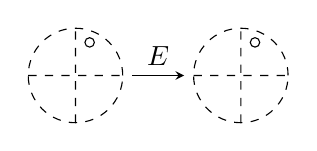
\begin{tikzpicture}[scale=0.6]
                \begin{scope}
                    \draw [dashed]
                        circle (1cm)
                        (0,-1) -- (0,1)
                        (-1,0) -- (1,0)
                    ;
                    \draw (0.3,0.7) circle (1mm);
                \end{scope}
                \draw [-stealth] (1.2,0) -- node[above]{$E$} (2.3,0);
                \begin{scope}[xshift=3.5cm]
                    \draw [dashed]
                        circle (1cm)
                        (0,-1) -- (0,1)
                        (-1,0) -- (1,0)
                    ;
                    \draw (0.3,0.7) circle (1mm);
                \end{scope}
            \end{tikzpicture}
            \caption{$E$.}
            \label{fig:stereographicElema}
        \end{subfigure}
        \begin{subfigure}[b]{0.32\linewidth}
            \centering
            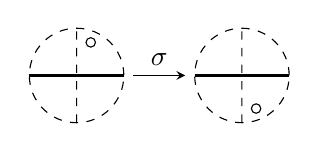
\begin{tikzpicture}[scale=0.6]
                \begin{scope}
                    \draw [dashed]
                        circle (1cm)
                        (0,-1) -- (0,1)
                    ;
                    \draw [very thick] (-1,0) -- (1,0);
                    \draw (0.3,0.7) circle (1mm);
                \end{scope}
                \draw [-stealth] (1.2,0) -- node[above]{$\sigma$} (2.3,0);
                \begin{scope}[xshift=3.5cm]
                    \draw [dashed]
                        circle (1cm)
                        (0,-1) -- (0,1)
                    ;
                    \draw [very thick] (-1,0) -- (1,0);
                    \draw (0.3,-0.7) circle (1mm);
                \end{scope}
            \end{tikzpicture}
            \caption{$\sigma$.}
            \label{fig:stereographicElemb}
        \end{subfigure}
        \begin{subfigure}[b]{0.33\linewidth}
            \centering
            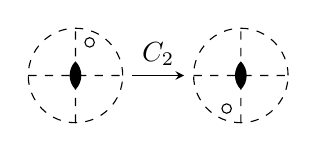
\begin{tikzpicture}[scale=0.6]
                \begin{scope}
                    \draw [dashed]
                        circle (1cm)
                        (0,-1) -- (0,1)
                        (-1,0) -- (1,0)
                    ;
                    \fill [scale=0.3] (90:1)
                        arc[start angle=135,end angle=225,radius=1.41cm]
                        arc[start angle=-45,end angle=45,radius=1.41cm]
                    ;
                    \draw (0.3,0.7) circle (1mm);
                \end{scope}
                \draw [-stealth] (1.2,0) -- node[above]{$C_2$} (2.3,0);
                \begin{scope}[xshift=3.5cm]
                    \draw [dashed]
                        circle (1cm)
                        (0,-1) -- (0,1)
                        (-1,0) -- (1,0)
                    ;
                    \fill [scale=0.3] (90:1)
                        arc[start angle=135,end angle=225,radius=1.41cm]
                        arc[start angle=-45,end angle=45,radius=1.41cm]
                    ;
                    \draw (-0.3,-0.7) circle (1mm);
                \end{scope}
            \end{tikzpicture}
            \caption{$C_n$.}
            \label{fig:stereographicElemc}
        \end{subfigure}\\[1em]
        \begin{subfigure}[b]{0.4\linewidth}
            \centering
            \begin{tikzpicture}[scale=0.6]
                \begin{scope}
                    \draw [dashed]
                        circle (1cm)
                        (0,-1) -- (0,1)
                        (-1,0) -- (1,0)
                    ;
                    \node [regular polygon,regular polygon sides=4,fill,inner sep=2mm,scale=0.3] {};
                    \draw (0.3,0.7) circle (1mm);
                \end{scope}
                \draw [-stealth] (1.2,0) -- node[above]{$C_4$} ++(1.1,0);
                \begin{scope}[xshift=3.7cm]
                    \draw (-1.1,-1.2) -- ++(-0.1,0) -- ++(0,2.4) -- ++(0.1,0);
                    \draw (1.1,-1.2) -- ++(0.1,0) -- ++(0,2.4) -- ++(-0.1,0);
                    \draw [dashed]
                        circle (1cm)
                        (0,-1) -- (0,1)
                        (-1,0) -- (1,0)
                    ;
                    \node [regular polygon,regular polygon sides=4,fill,inner sep=2mm,scale=0.3] {};
                    \draw (0.7,-0.3) circle (1mm);
                \end{scope}
                \draw [-stealth] (5.1,0) -- node[above]{$\sigma_h$} ++(1.1,0);
                \begin{scope}[xshift=7.4cm]
                    \draw [dashed]
                        circle (1cm)
                        (0,-1) -- (0,1)
                        (-1,0) -- (1,0)
                    ;
                    \node [regular polygon,regular polygon sides=4,fill,inner sep=2mm,scale=0.3] {};
                    \draw (0.7,-0.3) coordinate (x)
                        ([xshift=-0.7mm,yshift=-1mm]x) -- ++(1.4mm,2mm)
                        ([xshift=0.7mm,yshift=-1mm]x) -- ++(-1.4mm,2mm)
                    ;
                \end{scope}
    
                \draw [-stealth] (0,1.3) -- ++(0,0.6) -- node[above]{$S_4$} ++(7.4,0) -- ++(0,-0.6);
            \end{tikzpicture}
            \caption{$S_n$.}
            \label{fig:stereographicElemd}
        \end{subfigure}
        \begin{subfigure}[b]{0.4\linewidth}
            \centering
            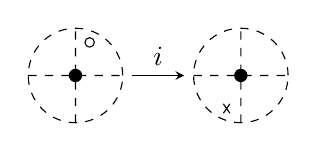
\begin{tikzpicture}[scale=0.6]
                \begin{scope}
                    \draw [dashed]
                        circle (1cm)
                        (0,-1) -- (0,1)
                        (-1,0) -- (1,0)
                    ;
                    \node [circle,fill,inner sep=2mm,scale=0.3] {};
                    \draw (0.3,0.7) circle (1mm);
                \end{scope}
                \draw [-stealth] (1.2,0) -- node[above]{$i$} (2.3,0);
                \begin{scope}[xshift=3.5cm]
                    \draw [dashed]
                        circle (1cm)
                        (0,-1) -- (0,1)
                        (-1,0) -- (1,0)
                    ;
                    \node [circle,fill,inner sep=2mm,scale=0.3] {};
                    \draw (-0.3,-0.7) coordinate (x)
                        ([xshift=-0.7mm,yshift=-1mm]x) -- ++(1.4mm,2mm)
                        ([xshift=0.7mm,yshift=-1mm]x) -- ++(-1.4mm,2mm)
                    ;
                \end{scope}
            \end{tikzpicture}
            \caption{$i$.}
            \label{fig:stereographicEleme}
        \end{subfigure}
        \caption{Stereographic projections of the elementary symmetry operations.}
        \label{fig:stereographicElem}
    \end{figure}
    \item Principal $C_n$ axis: The $C_n$ axis for which $n$ is the highest.
    \begin{itemize}
        \item In a stereographic projection, the $C_n$ axis is the one that is perpendicular to the working area (goes in/out of the page).
    \end{itemize}
    \item Example: Give the symmetry elements of \ce{NH3}.
    \begin{itemize}
        \item $C_3$ axis, 3 $\sigma_v$ mirror planes (denoted $\sigma_v$, $\sigma_v'$, and $\sigma_v''$).
        \item The symmetry operations are $E$, $C_3$, $C_3^2$, $\sigma_v$, $\sigma_v'$, and $\sigma_v''$. These operations form the $C_{3v}$ point group.
    \end{itemize}
    \item Direct products of symmetry operations: $YX=Z$ means "operation $X$ is carried out first and then operation $Y$," giving the same net effect as would the carrying out of the single operation $Z$.
    \begin{itemize}
        \item If $YX=XY=Z$, then the two operations $Y$ and $X$ commute.
    \end{itemize}
    \item What is the direct product of $C_2$ and $\sigma_h$?
    \begin{itemize}
        \item $\sigma_hC_2=S_2=i$. They do commute.
    \end{itemize}
    \item Do $C_4$ and $\sigma_{x,z}$ commute? Take the plane of this page as $xy$.
    \begin{itemize}
        \item They do not (determine by drawing out both sets of stereographic projections).
    \end{itemize}
    \item Don't get careless, Steven. This is easy, but it's also easy to make easy mistakes.
    \item New symmetry operations \emph{of your group} are generated by taking the direct product of two.
\end{itemize}



\section{Point Groups}
\begin{itemize}
    \item \marginnote{9/30:}The symmetry operations that apply to a given molecule collectively possess the properties of a mathematical \textbf{group}.
    \item \textbf{Group}: A set of symmetry operations that satisfy the following conditions.
    \begin{itemize}
        \item \emph{Closure}: All binary products must be in the group, i.e., the product of any two operators must also be a member of the group.
        \item \emph{Identity}: Must contain an identity, i.e., $E$ must be part of the group.
        \item \emph{Inverse}: All elements must have an inverse in the group, and they must commute with their inverse.
        \item \emph{Associativity}: The associative law $(A\cdot B)\cdot C=A\cdot(B\cdot C)$ must hold.
    \end{itemize}
    \item \textbf{Abelian} (group): A group in which all direct products commute.
    \begin{itemize}
        \item Not all groups are Abelian.
    \end{itemize}
    \item Question: Do $C_3$ and $\sigma_v$ form a group?
    \begin{itemize}
        \item No: No identity (for example).
        \item Wuttig draws out a stereographic projection for $C_3\cdot\sigma_v$ and overlays the first and last picture, showing that $C_3\cdot\sigma_v$ is a reflection over a new mirror plane $\sigma_v'$.
        \item $C_3$ and $\sigma_v$ do \textbf{generate} the set of operations $E,C_3,C_3^2,\sigma_v,\sigma_v',\sigma_v''$, which collectively form the \textbf{point group} $\bm{C_{3v}}$.
    \end{itemize}
    \item To prove something on a pset or exam, it's probably a good idea to do it in terms of stereographic projections!
    \item \textbf{Point group}: A group such that at least one point in space is invariant to all operations in the group.
    \item \textbf{Group order}: The number of symmetry operations in the group. \emph{Denoted by} $\bm{h}$.
    \item Table activity: Finding $E$, principal $C_n$, $\sigma$, $C_2\perp C_n$, $C_n$ position relative to $\sigma$ (collinear or perpendicular), and $i$ for various point groups.
    \begin{itemize}
        \item These properties are the ones that distinguish each point group from every other point group.
    \end{itemize}
    \item Notes on the pedagogy: Animations and/or tangible models should be used to discuss this stuff. PowerPoint slides are definitely the way to go --- far more tangible tools; blackboard should be a supplement. It is key to be careful what you say (\emph{element} and \emph{operation} must be consistently used). Dr. Wuttig is skipping a lot of key points (like naming point groups).
    \item Developing a flow chart that distinguishes between $D_{nh}$, $D_{nd}$, $D_n$, $C_{nh}$, $C_{nv}$, $C_n$, and $S_n$.
\end{itemize}




\end{document}